\documentclass[parskip=half,DIV=14]{scrartcl}\usepackage[]{graphicx}\usepackage[]{color}
%% maxwidth is the original width if it is less than linewidth
%% otherwise use linewidth (to make sure the graphics do not exceed the margin)
\makeatletter
\def\maxwidth{ %
  \ifdim\Gin@nat@width>\linewidth
    \linewidth
  \else
    \Gin@nat@width
  \fi
}
\makeatother

\definecolor{fgcolor}{rgb}{0.345, 0.345, 0.345}
\newcommand{\hlnum}[1]{\textcolor[rgb]{0.686,0.059,0.569}{#1}}%
\newcommand{\hlstr}[1]{\textcolor[rgb]{0.192,0.494,0.8}{#1}}%
\newcommand{\hlcom}[1]{\textcolor[rgb]{0.678,0.584,0.686}{\textit{#1}}}%
\newcommand{\hlopt}[1]{\textcolor[rgb]{0,0,0}{#1}}%
\newcommand{\hlstd}[1]{\textcolor[rgb]{0.345,0.345,0.345}{#1}}%
\newcommand{\hlkwa}[1]{\textcolor[rgb]{0.161,0.373,0.58}{\textbf{#1}}}%
\newcommand{\hlkwb}[1]{\textcolor[rgb]{0.69,0.353,0.396}{#1}}%
\newcommand{\hlkwc}[1]{\textcolor[rgb]{0.333,0.667,0.333}{#1}}%
\newcommand{\hlkwd}[1]{\textcolor[rgb]{0.737,0.353,0.396}{\textbf{#1}}}%

\usepackage{framed}
\makeatletter
\newenvironment{kframe}{%
 \def\at@end@of@kframe{}%
 \ifinner\ifhmode%
  \def\at@end@of@kframe{\end{minipage}}%
  \begin{minipage}{\columnwidth}%
 \fi\fi%
 \def\FrameCommand##1{\hskip\@totalleftmargin \hskip-\fboxsep
 \colorbox{shadecolor}{##1}\hskip-\fboxsep
     % There is no \\@totalrightmargin, so:
     \hskip-\linewidth \hskip-\@totalleftmargin \hskip\columnwidth}%
 \MakeFramed {\advance\hsize-\width
   \@totalleftmargin\z@ \linewidth\hsize
   \@setminipage}}%
 {\par\unskip\endMakeFramed%
 \at@end@of@kframe}
\makeatother

\definecolor{shadecolor}{rgb}{.97, .97, .97}
\definecolor{messagecolor}{rgb}{0, 0, 0}
\definecolor{warningcolor}{rgb}{1, 0, 1}
\definecolor{errorcolor}{rgb}{1, 0, 0}
\newenvironment{knitrout}{}{} % an empty environment to be redefined in TeX

\usepackage{alltt}
\usepackage{amsmath}
\usepackage[automark]{scrpage2} 
\usepackage{hyperref}
\usepackage[backend=bibtex]{biblatex}
\usepackage[section]{placeins}

\addbibresource{documentation.bib}
\title{Documentation of MOCK and PESA-II Implementation in R}
\author{Dennis Assenmacher, Christian Homberg}

\let\endtitlepage\relax
 
\makeatletter
\renewcommand{\maketitle}{
   \clearscrheadfoot
   \cfoot{\pagemark}
   \begin{titlepage}
   
   \thispagestyle{scrheadings}
   \begin{center}
   \vspace*{-2cm}
   
\includegraphics{wwu}
   \vspace{8pt}
   \hrule
   \vspace{15pt}
       {\Huge \@title}
 
   \vspace{\parskip}
 
   {\Large \@author}
 
   \@date
   \end{center}
   \end{titlepage}
}
\makeatother
\IfFileExists{upquote.sty}{\usepackage{upquote}}{}
\begin{document}



\maketitle

\section{Introduction}
This documentation provides information about the R packages MOCK and PESA-II. Both packages were created as part of a seminar on advanced R in 2015/2016. The main goal of this documentation is to give insights in how the MOCK algorithm, proposed by \textcite{handl} works in general, how it is implemented in R/C++ and how it can be used in order to get both analytical and visual results. Currently the packages are not available at the Comprehensive R Archive Network (CRAN). Therefore we suggest to install them via devtools:
\begin{knitrout}
\definecolor{shadecolor}{rgb}{0.969, 0.969, 0.969}\color{fgcolor}\begin{kframe}
\begin{alltt}
\hlstd{devtools}\hlopt{::}\hlkwd{install_github}\hlstd{(}\hlstr{"https://github.com/Dennis1989/MOCK"}\hlstd{,}\hlstr{"MOCK"}\hlstd{)}

\hlstd{devtools}\hlopt{::}\hlkwd{install_github}\hlstd{(}\hlstr{"https://github.com/Dennis1989/MOCK"}\hlstd{,}\hlstr{"PESAII"}\hlstd{)}
\end{alltt}
\end{kframe}
\end{knitrout}

Within the following chapters we will explain the basic concepts of multi-objective clustering as well as the concepts of MOCK and different evolutionary multiobjective algorithms (EMOAs). We additionally provide some implementation details and how MOCK can be adjusted. Finally we focus on implementation decisions as well as benchmarking and conclude with working examples and provide an outlook.
\section{Multi-objective clustering}
Data clustering in general can be informally described as the process of finding homogeneous groups of data objects. The question which arises is how we can assess the quality of clustering solutions and therefore seperate good solutions from bad ones. One would argue that this is only possible by having access to external expert knowledge. Since clustering is an unsupervised learning method, such knowledge is rarely available. Therefore internal clustering criteria are applied. \textcite{handl2007} describe it formally as an optimization problem: 
\begin{displaymath}
P(C^*) = \underset{C\in\Omega}{\min}\ P(C)
\end{displaymath}

where $C$ is the set of all possible cluster solutions and $P:\Omega \rightarrow R$ an internal clustering criterion function. 

In general one single criterion function would not be able to detect all possible cluster structures \cite{handl2007}. Therefore the need of reformulating the one-dimensional problem into a multi-dimensional optimization task is evident:

\begin{displaymath}
P_t(C^*) = \underset{C\in\Omega}{\min}\ P_t(C), t=1,...,n
\end{displaymath}

The most prominent clustering critera are based on either achieving a compact solution or a connected one. Compact clusters try to identify solutions which hold the variation between cluster data as small as possible. In this context the \textit{k}-means algorithm\cite{kmeans} and agglomerative clustering are frequently used. Connected clustering solutions on the other hand focus on grouping neighboring data together into one cluster. Average linkage tends to enforce the creation of those closely connected chains. However, it should be emphazised that it is not possible to detect all structures by only optimizing either compactness or connectedness. Therefore MOCK defines a multidimensional optimization task as stated above by optimizing in terms of compactness and connectedness. In the following section we will describe MOCK's evolutionary approach in detail.

\section{MOCK}

Basically MOCK can be separated into two distinct phases: The clustering phase and the automatic determination of clustering solutions. In the following sections we describe each of those phases in detail.

\subsection{Clustering Phase}
First of all, the clustering phase uses an evolutionary algorithm in order to obtain distinct nondominated cluster solutions which approximate the true pareto front. In case of MOCK, Handl suggests to use the pareto envelope-based selection algorithm version 2 (PESA-II). However, as a lot of different EMOA's currently exist, we try to describe the clustering phase more generally in order to be able to adapt MOCK to other EMOA's like SMS-EMOA or NSGA-II. A list of state of the art algorithms and their comparison can be inspected in \cite{comparison}.

All EMOAs follow the basic cycle of biological evolution: reproduction, mutation, recombination and selection. The difference between each algorithm lies in the operators used for these different steps. In order to be able to adapt MOCK to different EMOAs it is necessary to describe these operators as well as the problem representation and the objective functions used to determine the solution fitness.
\subsubsection{Objective functions}

As already described in the previous chapter, MOCK uses two contradicting clustering objectives based on compactness and connectedness.

To determine compactness, MOCK determines the overall deviation for each cluster solution. Informally it can be described as the sum of all summed distances between each data-object and their corresponding cluster center.

Formally we specify it as:

\begin{displaymath}
\operatorname{DEV}(C) = \sum_{C_k \in C} \sum_{i \in C_k} \delta(i,\mu_k)
\end{displaymath}

where C is denoted as the set of all clusters and $\mu_k$ the central point of one cluster $C_k$.

The second objective function, which measures the connectedness, is called connectivity. Informally it measures the degree to which neighboring data points have been placed in the same cluster\cite{handl}:


\begin{displaymath}
\operatorname{CONN}(C) = \sum_{i=1}^N \sum_{j=1}^L (x_{i,nn_{ij}})
\end{displaymath}

\begin{center}
$x_{r,s}$ = $\frac{1}{j}$, if $\notin C_k:r\in C_k$ and $s\in C_k$
\end{center}

where $nn_{i,j}$ is the j'th nearest neighbor of i. The formula indicates that the overall connectivity increases if neighboring points are not in the same cluster. Therefore the objective should be minimized as well as the overall deviation.

\subsubsection{Representation}
Each clustering solution is represented as a locus-based adjacency representation \cite{handl}. Each cluster solution contains N genes, where one gene is equivalent to one data-object within a certain cluster problem. Each gene can take a value $\in 1..N$. If gene $i$ takes the value $j$, we can interpret it as an existing link between $i$ and $j$. Since we can implement this within a simple numeric vector and also are able to simply apply mutation and crossover operators, this representation seems to work well for MOCK. Note that there is some computational effort necessary to determine which data objects belong to the same cluster. Handl argues that this decoding step can be achieved in linear time \cite{handl}.

A visualisation of the locus based adjacency scheme can be found in \ref{fig:locus}.

\begin{figure}[h]
\begin{center}
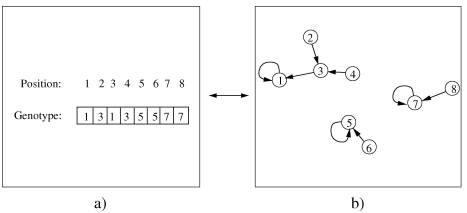
\includegraphics{figure/locus.png}
\caption{Locus-based adjacency scheme from \cite{handl2007}  }
\label{fig:locus}
\end{center}
\end{figure}

\subsubsection{Recombination}
As recombination operator Handl uses uniform crossover. Two parents are first selected and a random masking vector is applied in order to determine which gene is transferred to the child.

\subsubsection{Mutation}
In order to reduce the search space for mutation, MOCK makes use of restricted nearest-neighbor mutation. The basic idea is to restrict possible mutations in a way that one gene can only be connected to one of its $L$ nearest neighbors. A great advantage of this approach is that this drastically reduces the search space from $N^N$ to $L^N$, where $L<N$ and also saves a lot of computation time since the nearest neighbor matrix only has to be calculated once (we do not change the position of data objects). Additionaly we have to consider that shorter links are more favourable than longer links. Therefore, Handl defines the probability of mutation for a link $i\rightarrow j$ as:

\begin{displaymath}
p_m = \frac{1}{N} + (\frac{l}{N})^2
\end{displaymath}

where $j = nn_{il}$ (j is l'th nearest neighbor of i). It is obvious that a link $i\rightarrow h$ with $nn$ would be preffered.

The probability of mutation can be directly integrated into the precomputed nearest neighbor matrix. More information on implementation details can found within chapter 5.

\subsubsection{Initialization}
An important step within the MOCK algroithm is the creation of initial solutions. The main goal is to achieve a well spreaded initial solution front in order to be able to search the whole solution space. As described in chapter 2, different single objective cluster algorithms perform well under either compactness or connectedness. Therefore, half of the initial solutions are generated with \textit{k}-means, which performs well
under compactness, and the other half by generating connected solutions obtained from a minimum spanning tree. In both cases the same amount of solutions is created by conducting \textit{k}-means and respectively cutting the \textit{k}-largest edges of the minimum spanning tree where \textit{k} is iterated over 1 to maxCluster.
\subsection{Automatic determination of clustering solutions}
The previously introduced objective functions deviation and connectivity lead to a pareto front in two dimensional space. Since each point on the pareto front represents one non-dominated clustering solution (at least for the PESA-II implementation), it is not possible to identify one best solution in regard to the objective functions. Even more, the solutions differ in the amount of clusters (k), usually the deviation decreases as the connectivity and k increases. The solutions identified by MOCK during the clustering phase can therefore only be regarded as candidates which should be the object of further inspection, either by domain experts or by applying one of the many heuristic approaches for the determination of k in clustering theory. One approach which is also the basis for MOCK is to inspect the pareto front for a "knee", that is an area where the deviation greatly decreases while the connectivity does not increase much. Since the objective functions may be biased by the number of clusters, the inspection is conducted on a normalized pareto front. Furthermore, the MOCK pareto front is compared to reference fronts. These are generated by conducting MOCK on datasets with as similar characteristics as the original data as possible except for the existence of clusters. This data is generated uniformly within the eigenspace of the original data and back-transformed to its range. For each point of the pareto front the nearest Euclidean distance to any of the dominated control fronts is calculated, a measure called attainment score \ref{fig:attainment}. It can be expected that a large attainment score indicates a good solution since deviation and connectivity are especially good when compared to solutions on the control fronts with the same amount of clusters. By the same logic a plot of attainment scores and amount of clusters can help identify a set of potential best solutions\label{fig:attainment}. The local maxima in this plot build a set of promising candidates while the global maximum can point to the best solution. \cite{handl}



% \subsection{Summary}
% Within the current chapter we defined all operators which are necessary for running the MOCK algorithm during the clustering phase. In contrast to the original MOCK paper we do not only allow the usage of PESA-II as the underlying EMOA but provide the user with different options of selecting their favourite algorithm. Since we identified the fundamental operators, other EA's only need to be slightly adapted. We will explain these adoptions in case of SMS-EMOA in chapter 4.4. Next we will get an overview of the different EMOA's in general.
\section{Multi-Objective-Evolutionary-Algorithms (EMOA)}
The following section provides a brief introduction into three different EMOAs, since these are included and can be used within the MOCK package. It should be emphasized that we will not provide a detailed description of each algorithm but only explain the fundamental concepts. As we already defined the operators used by MOCK, we can integrate them into each algorithm.
\subsection{SMS-EMOA}
SMS-EMOA was introduced in 2008 by \textcite{smsemoa}. The basic idea of this algorithm is to apply the S-metric within its selection operator. The S-metric is a measure which determines the dominated hypervolume of an approximated Pareto front. Therefore the S-metric should be maximized. This maximization is realized by eleminating the solution with the lowest contribution to the dominated hypervolume in each generation. In order to apply SMS-EMOA within MOCK, we have to integrate our predefined operators. First of all we have to make sure that we initialize as much solutions as we need. Since SMS-EMOA starts with a fixed set of solutions and only deletes and creates one new solution in each generation, the amount of initial solutions is equivalent to the amount of final solutions. Next we have to apply reproduction and mutation. This can be achieved by selecting randomly two parents from the last solution set and create a child by calling \textit{crossoverMock} and mutating it via \textit{mutateMock}, provided within the MOCK-package. 

\subsection{NSGA-II}
In contrast to SMS-EMOAs $\mu + 1$ selection strategy, NSGA-II \cite{nsga2} makes use of an $\mu + \mu $ selection, so that for each iteration $\mu$ new individuals are generated and $\mu$ indivudials with the best fitness values are selected for the next generation. There are two different selection criteria within NSGA-II. First NSGA-II performs non-dominated sorting. Therefore all solutions are separated into different pareto layers. The second criteria is applied to the last non-dominated layer and is called crowded distance sorting. The crowding distance (CD) is a measure for the space around non-dominated solutions in which no other solution is found. All in all, applying CD enforces the selection of well spreaded solutions. For a detailed description of NSGA-II and the formalization of CD we suggest the original specification of NSGA-II \cite{nsga2}. 

\subsection{PESA-II}
In contrast to most of the standard EMOAs individual-based selection criteria, PESA-II follows a region-based approach that is the selection of a hyperbox rather than an individual \cite{pesa}. Also two populations are stored during the run: an internal population (IP) of fixed size which is used for exploring new solutions and an external population of limited size which is used to maintain and exploit good solutions. Basically the algorithm follows distinct steps after creating the initial population and storing it into EP:

\begin{enumerate}
\item IP is filled by selecting randomly a populated niche from the hypergrid and a random solution $s$ from that niche. Therefore highly populated areas do not contribute more than less populated areas.

\item All solutions in IP are processed by reproduction and variation.

\item If a solution in IP dominates any solution in EP, delete those dominated solutions from EP and add IP's solution to EP.

If a solution in IP is nondominated and EP is not full, add those solutions to EP. If EP is full only add the solution to EP if it is stored in a less crowded niche than any other solution. Therefore PESA-II encourages the exploration of the whole objective space. PESA-II is used within MOCK as the standard EMOA. One main advantage of PESA-II in that scenario is that IP determines the the number of evaluations per generation and EP the maximum amount of final solutions. This seperation is not present in the other algorithms.
\end{enumerate}

Especially step three ensures the generation of a well spreaded pareto front since only those nondominated solutions are added to the external population which are situated within a less crowded niche.  
\subsection{Other EMOAs}
As already indicated, it is straightforward to integrate other EMOAs into MOCK. The initialization of solutions, the representation and also the basic operators are already defined within the package and can be reused. All in all there are three steps which are necessary in order to adjust a EMOA.

\begin{enumerate}
\item  Generate the necessary amount of inital solutions
\item  Embed \textit{crossoverMock} into the algorithm
\item  Embed \textit{mutateMock} into the algorithm
\end{enumerate}

\section{Implementation}

In this chapter we explain some implementation details of the MOCK- as well as the
PESA-II package. We start by giving an overview of the repository design followed by a discussion of how performance issues were addressed.

\subsection{Repository overview}
Currently we provide the possibility to run MOCK with either PESA-II, NSGA-II or
SMS-EMOA. Since PESA-II is used within the original paper, it is defined as the stan-
dard algorithm. As there was no R Package implementing PESA-II available when the
seminar started, we decided to create an additional package PESA-II. Note that this
package does not depend on the MOCK package and can therefore be used indepen-
dently to solve any multiobjective optimization problem. Besides the two packages the github repository contains a third R folder “additions” that includes four files. These do not specifically belong to either package but are included in order to allow a reproduction of the results of this paper.

\subsection{Performance improvements}
Initially, both the MOCK objective and PESA-II were developed independently and entirely in R. Only the integration revealed that the performance of this implementation is insufficient. Using the profiler profvis (source: https://github.com/rstudio/profvis) we identified the most timeconsuming functions and implemented them in C++ using the Rcpp package. In the prioritization we also considered the estimated effort for the C++ implementation. Replacing one single line by dominatesC for example lead to speedups of several seconds. Below we list some of the most timeconsuming, frequently called, and important functions which were implemented in Rcpp:

\begin{itemize}
\item dominatesC
\item fastNonDominatedSortingR
\item decodeC
\item deviationC
\item connectivity
\item whichC
\item mutateC
\item mockFunctionC
\end{itemize}

One of the most frequently called functions in all EMOAs is mockFunctionC which is why we chose to implement the whole objective function in C++. Still, since with the default parameters the function is called 10.000 times per MOCK run-through it takes about 20\%-60\% of the runtime, depending on the parameters chosen. Yet, only the partial implementation of fastNonDominatedSortingR in C++ came along with similarly large performance improvements for SMS-EMOA. The following function call took 94.2s using the improved function compared to 366.7s using the function included in the nsga2R package.
\begin{knitrout}
\definecolor{shadecolor}{rgb}{0.969, 0.969, 0.969}\color{fgcolor}\begin{kframe}
\begin{alltt}
\hlkwd{mock}\hlstd{(}\hlkwc{data}\hlstd{=clusterData,}\hlkwc{L}\hlstd{=}\hlnum{10}\hlstd{,}\hlkwc{crossRae}\hlstd{=}\hlnum{0.7}\hlstd{,}\hlkwc{nGrid}\hlstd{=}\hlnum{10}\hlstd{,}\hlkwc{gens}\hlstd{=}\hlnum{10000}\hlstd{,}
     \hlkwc{method}\hlstd{=}\hlstr{"smsemoa"}\hlstd{,}\hlkwc{controlFronts}\hlstd{=}\hlnum{1}\hlstd{)}
\end{alltt}
\end{kframe}
\end{knitrout}
Even though the performance has already been drastically improved by implementing about 25\% of the code in C++, it is clear that there is still room for improvements. 



\section{Benchmarking}
Our benchmarking approach consists of three different methods:
\begin{enumerate}
\item Comparison of pareto fronts with original Mock tool (source to original tool).
\item Comparison of pareto fronts with other “standard” clustering algorithms.
\item Comparison of pareto fronts and clustering solutions between different EMOAs.
\end{enumerate}
The methods and their results are presented in the subsequent subsections.

\subsection{Comparison with original Mock tool}

In order to legitimate our implementation of MOCK we compare pareto fronts obtained by the PESA-II implementation with the results of the original Mock tool by Handl. This visual benchmark is conducted for the same datasets and where possible for the same parameters. 
The results are depicted in figure \ref{fig:comparison}.

\begin{figure}[h]
\begin{center}
\includegraphics[scale=0.75]{figure/comparisonMockTool.pdf}
\caption{Comparison between MOCK package and original Mock tool}
\label{fig:comparison}
\end{center}
\end{figure}

A superficial visual inspection of the benchmarks reveals that both implementations produce very similar pareto fronts, both for the unnormalized and the normalized plots. In the following we will only consider the unnormalized cases. A normalization without distorting the aspect ratio of each pareto front is not possible since usually the only common point in both fronts is the one cluster solution.

The dataset which produces the most similar results is Square1. In this case both pareto fronts overlap almost completely. On the first look, deviations between the fronts could be due to different random numbers generated during runtime. However, this benchmark shows the same characteristics as the others, only much less distinct. For one, our R implementation mostly dominates the original Mock tool for solutions with many clusters while the Mock tool tends to find more and better few-cluster solution. Also, just as for the Long1 dataset, the Mock tool finds more solutions at the right lower end of the pareto front. However, these are partially dominated by the R solutions and this observation does not apply to the Spiral dataset. Besides different random numbers there are two  more likely reasons why the implementations don’t produce more similar pareto fronts. Firstly, some MOCK parameters used in the original tool are unknown and can therefore be only guessed. We default to the parameters proposed in \cite{handl2007} (with $k_{User}=50$) which may differ from the actual implementation. Secondly, although our work is based on the pseudo-code and descriptions presented in \cite{handl2007} we cannot guarantee equality to the original implementation.

\subsection{Comparison with standard clustering algorithms}

Although we just showed that our MOCK implementation produces very similar solutions as the MOCK tool by Handl, as in the original paper\cite{handl}, we compare our PESA-II implementation with the \textit{k}-means algorithm as well as single and average linkage agglomerative clustering. Especially \textit{k}-means (compactness) and single linkage agglomerative clustering (connectivity) perform well under MOCK’s two objective functions and are therefore suitable for benchmarking the entire pareto front.
\begin{figure}[h]
\begin{center}
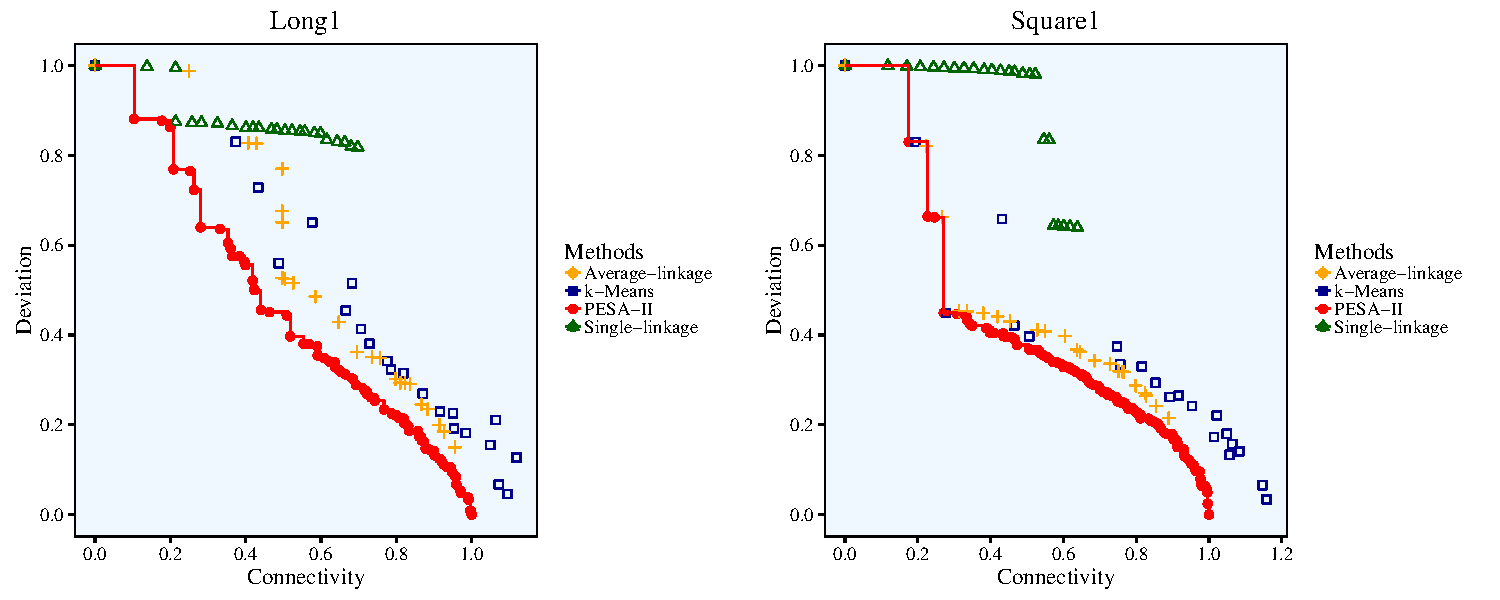
\includegraphics[scale=0.65]{figure/Long1Square1Benchmark.pdf}
\caption{Comparison of pareto front with standard algorithms}
\label{fig:standard}
\end{center}
\end{figure}

The analysis of the results does not reveal new insights since for the Long1 and Spiral datasets the benchmarks resemble remarkably those presented by \textcite{handl2005}(see Figure \ref{fig:standard}). Given the very minor deviations to the original MOCK tool (see section 6.1) this was expected. Therefore we reference to the benchmarks applied previously by \textcite{handl}\cite{handl2005}\cite{handl2007}.


\subsection{Comparison between different EMOAs}

Originally MOCK was intended to be used in combination with PESA-II. Since we added two more algorithms, namely NSGA-II and SMS-EMOA, a performance evaluation would show which algorithm works best. However, in order to achieve an objective result, we need to carefully specify MOCK's parameter for each individual algorithm. Because of their different selection strategies it is not possible to use the same number of generations. SMS-EMOA for example only generates one individual per iteration while NSGA-II generates $\mu$ new offsprings. Also we have to ensure, in terms of comparability, that the maximum number of solutions at our approximated pareto front is the same for each algorithm. Figure \ref{fig:amount} states the amount of evaluations per generation and the parameter which determines the maximum amount of solutions, for each of the three algorithms.


\begin{figure}[h]
\begin{center}
\begin{tabular}{|c|c|c|c|}
\hline 
• & PESA-II & NSGA-II & SMS-EMOA \\ 
\hline 
\#eval per generation & IPMax & \mu & 1 \\ 
\hline 
max solutions & EPMax & \mu & \mu \\ 
\hline 
\end{tabular}
\caption{Comparison EMOAs: \#evaluations and \#solutions}
\label{fig:amount}
\end{center}

\end{figure}




By choosing one algorithm and setting fixed parameters we can adjust the settings for the other algorithms in a way that the overall amount of evaluations, namely the call of the mock function is the same for all of them. Therefore the recommended parameter setup for PESA-II within the original MOCK paper is used \cite{handl2007}. The following Figure \ref{fig:parameter} shows the parameter specification for each algorithm.

NSGA-II and SMS-EMOA do not differentiate between internal and external population as PESA-II does. Instead they specify $\mu$ in order to determine how many solutions will be available within the approximated pareto front. Using this specification we ensure that each algorithm executes 10,000 evaluations.

\begin{figure}[h]
\begin{center}
\begin{tabular}{|c|c|c|c|}
\hline 
• & PESA-II & NSGA-II & SMS-EMOA \\ 
\hline 
\#generations & 1000 & 100 & 10000 \\ 
\hline 
EP & 100 & X & X \\ 
\hline 
IP & 10 & X & X \\ 
\hline 
gridsize & 10 & X & X \\ 
\hline 
L & 10 & 10 & 10 \\ 
\hline 
\mu & X & 100 & 100 \\ 
\hline 
p_m & 0.7 & 0.7 & 0.7 \\ 
\hline 
\#evaluations & IP * \#gen & \#gen * \mu & \#gen * \mu \\ 
\hline 
\end{tabular}
\caption{Parameter specification for each EMOA}
\label{fig:parameter}
\end{center}
\end{figure}
Within the overall benchmark process we used three different datasets which were already analyzed in the latest publication of MOCK \cite{handl2007}: long1, square1 and spiral. \textcite{zitzler} propose three different quality indicators for a multiobjective optimization problem:

\begin{enumerate}
\item The distance of the approximated pareto front to the true pareto front should be minimized
\item Solutions should be well distibuted
\item For each objective a wide range of values should be achieved.
\end{enumerate}


Since the true pareto front is unknown, we evaluate our solutions by comparing them to each other and to the solutions from the original MOCK-Tool. Figure \ref{fig:comp} shows for each dataset the approximated pareto fronts of the three different algoithms in a normalized and unnormalized format.
\begin{figure}[!htb]
\begin{center}
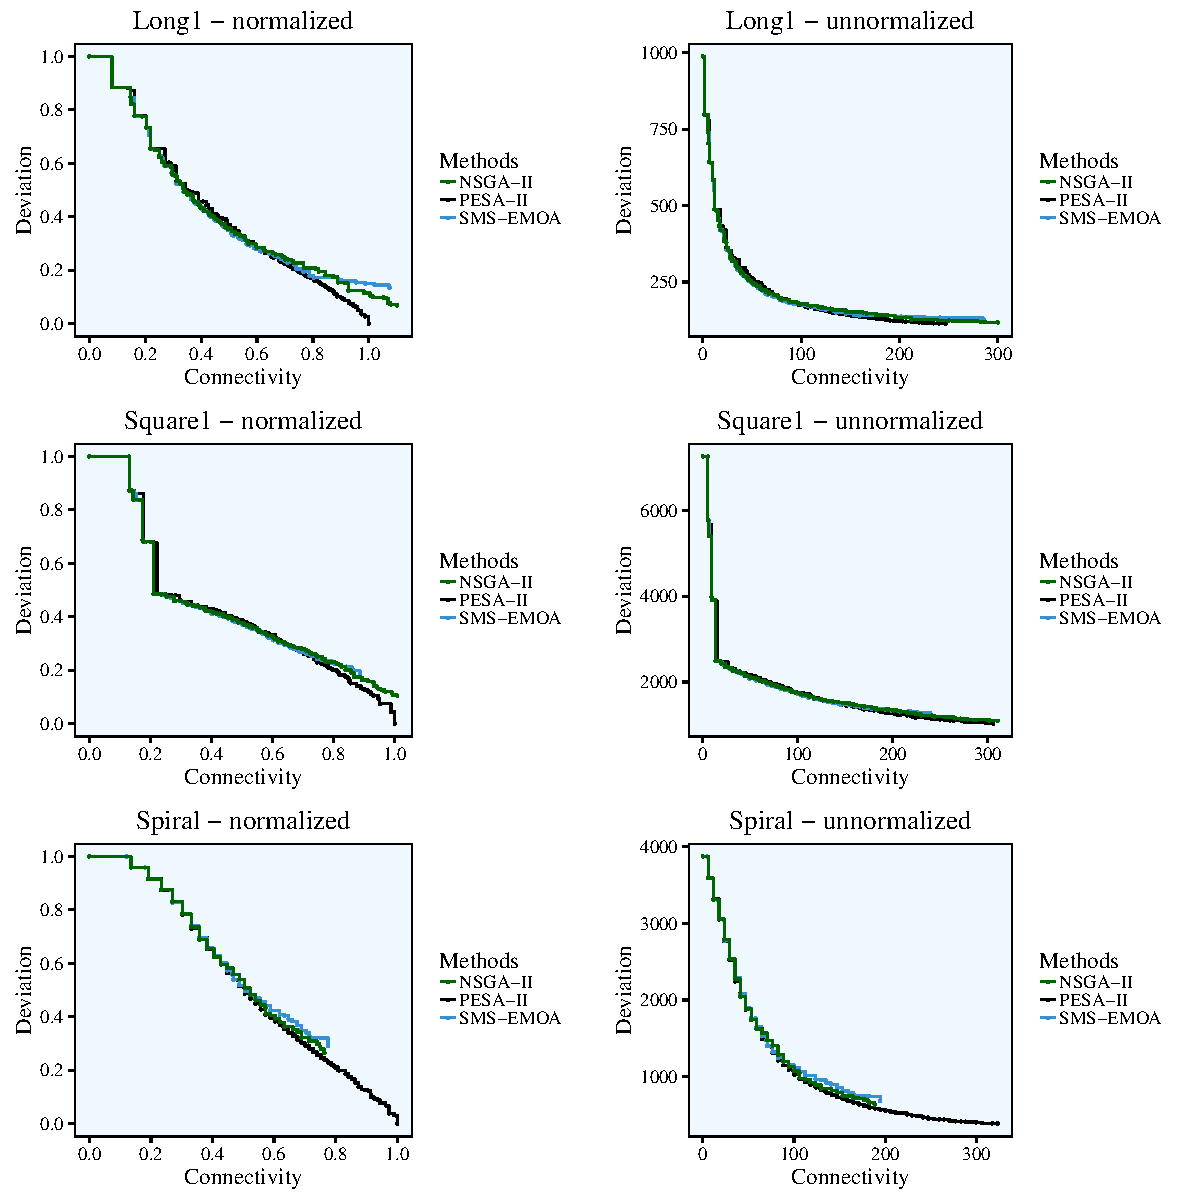
\includegraphics[scale=0.70]{figure/Comparison.pdf}
\caption{From top to bottom: \emph{long1}, \emph{suqare1} and \emph{spiral} dataset: normalized (left) and unnormalized(right) plots}
\label{fig:comp}
\end{center}
\end{figure}


At first sight none of those three algorithms' pareto fronts is completely dominated by any other. However at least for our test runs NSGA-II has the lowest share of the oveall pareto front for all three data sets. Also it is evident that PESA-II finds the best solutions for a high number of clusters and outperforms the other ones in most cases.

By putting all 300 solutions into one single pareto front and deleting dominated points the overall contribution of each algorithm to this front can be determined. For the long and square dataset the contribution of SMS-EMOA algorithm to the overall pareto front is higher than the contribution of the other algorithms.

\begin{figure}[h]
\begin{center}
\begin{tabular}{|c|c|c|c|}
\hline 
• & PESA-II & NSGA-II & SMS-EMOA \\ 
\hline 
long & 37.64\% & 21.35\% &  41.01\% \\ 
\hline 
square &34.16\%& 16.77\% & 49.07\% \\ 
\hline 
spiral & 47.54\% & 15.85\% & 36.61\% \\ 
\hline 
\end{tabular} 
\caption{Share of solutions of overall pareto front}
\end{center}
\end{figure}


\section{Usage}
Within this chapter we want to provide guidelines of how to use the functions of the MOCK and PESA-II package by analyzing an exemplary dataset. For our purpose we use the Square1 dataset which was already analyzed in \cite{handl2007}. First of all we load the datset as a matrix into R:




\begin{knitrout}
\definecolor{shadecolor}{rgb}{0.969, 0.969, 0.969}\color{fgcolor}\begin{kframe}
\begin{alltt}
\hlstd{square} \hlkwb{=} \hlkwd{read.csv}\hlstd{(}\hlstr{"PATH\textbackslash{}\textbackslash{}square1.data"}\hlstd{,}\hlkwc{header} \hlstd{= F,} \hlkwc{sep} \hlstd{=} \hlstr{" "}\hlstd{)[,}\hlnum{1}\hlopt{:}\hlnum{2}\hlstd{]}
\end{alltt}
\end{kframe}
\end{knitrout}

Now it is time to run MOCK. As already described in the previous chapter, we first have to choose between one of the three different EMOA's which should be used during the clustering phase. First we decide to use PESA-II. Therefore we have to provide all necessary parameters. In our case we use the parameters used for analyzing the data in section six. 



\begin{knitrout}
\definecolor{shadecolor}{rgb}{0.969, 0.969, 0.969}\color{fgcolor}\begin{kframe}
\begin{alltt}
\hlstd{solution} \hlkwb{=} \hlkwd{mock}\hlstd{(}\hlkwc{data} \hlstd{= square,}\hlkwc{L} \hlstd{=} \hlnum{10}\hlstd{,}\hlkwc{crossRate} \hlstd{=} \hlnum{0.7}\hlstd{,}\hlkwc{nGrid} \hlstd{=} \hlnum{10}\hlstd{,}
           \hlkwc{gens} \hlstd{=} \hlnum{1000}\hlstd{,}\hlkwc{method}\hlstd{=}\hlstr{"pesa"}\hlstd{,}\hlkwc{controlFronts} \hlstd{=} \hlnum{1}\hlstd{,}\hlkwc{epMax} \hlstd{=} \hlnum{100}\hlstd{,}
           \hlkwc{ipMax} \hlstd{=} \hlnum{10}\hlstd{,}\hlkwc{maxCluster}\hlstd{=}\hlnum{50}\hlstd{)}
\end{alltt}
\end{kframe}
\end{knitrout}


After this call we obtain a mock object which contains all information gathered through the run. Probably the most interesting attribute is the list of solutions. It can be accessed via calling  

\begin{knitrout}
\definecolor{shadecolor}{rgb}{0.969, 0.969, 0.969}\color{fgcolor}\begin{kframe}
\begin{alltt}
\hlstd{solution}\hlopt{$}\hlstd{sol}
\end{alltt}
\end{kframe}
\end{knitrout}

Each entry within the list represents one cluster solution and contains the corresponding encoding as well as its fitness values for deviation and connectivity. For post-processing purposes it is needed to decode the adjacency encoding to get the true cluster assignments for each data-object. Therefore we can decode the cluster by calling the \textit{decodeC} function:

\begin{knitrout}
\definecolor{shadecolor}{rgb}{0.969, 0.969, 0.969}\color{fgcolor}\begin{kframe}
\begin{alltt}
\hlkwd{decodeC}\hlstd{(solution}\hlopt{$}\hlstd{sol[[}\hlnum{1}\hlstd{]]}\hlopt{$}\hlstd{param)}
\end{alltt}
\end{kframe}
\end{knitrout}

However for a quick peak at the results (see Figure \ref{fig:printpareto}) we can also use the build-in visualization function of the MOCK package. To have a look at the approximated pareto front we can call

\begin{knitrout}
\definecolor{shadecolor}{rgb}{0.969, 0.969, 0.969}\color{fgcolor}\begin{kframe}
\begin{alltt}
\hlkwd{printParetoFront}\hlstd{(solution,}\hlkwc{method}\hlstd{=}\hlstr{"fronts"}\hlstd{,}\hlkwc{labelType}\hlstd{=}\hlstr{"none"}\hlstd{)}
\end{alltt}
\end{kframe}
\end{knitrout}

\begin{figure}
\begin{center}
\begin{knitrout}
\definecolor{shadecolor}{rgb}{0.969, 0.969, 0.969}\color{fgcolor}

{\centering 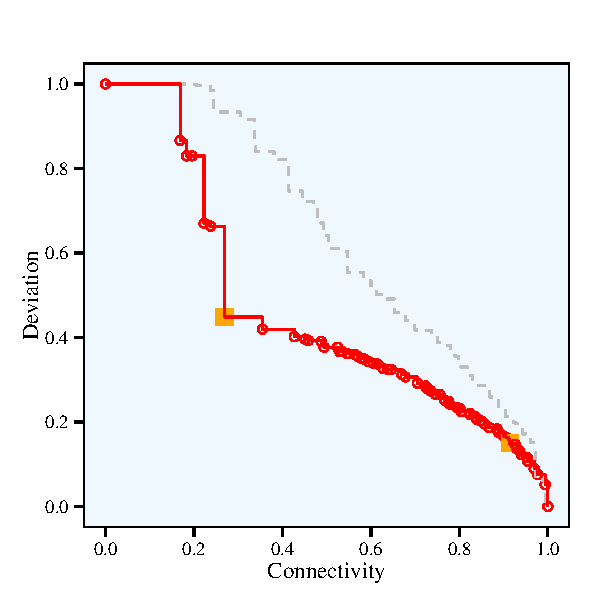
\includegraphics[width=\maxwidth]{figures/plots-printFront-1} 

}



\end{knitrout}
\caption{Approximated pareto front for \textit{Square1} dataset}
\label{fig:printpareto}
\end{center}
\end{figure}

Here we also include the reference fronts. If those additional fronts should not be displayed we can simply omit them by leaving out the method attribute. Next we can have a look at the attainment plot (\ref{fig:attainment}) in order to identify promising cluster solutions. Therefore 
\begin{knitrout}
\definecolor{shadecolor}{rgb}{0.969, 0.969, 0.969}\color{fgcolor}\begin{kframe}
\begin{alltt}
\hlkwd{printAttainmentScore}\hlstd{(solution)}
\end{alltt}
\end{kframe}
\end{knitrout}
\begin{figure}
\begin{center}
\begin{knitrout}
\definecolor{shadecolor}{rgb}{0.969, 0.969, 0.969}\color{fgcolor}

{\centering 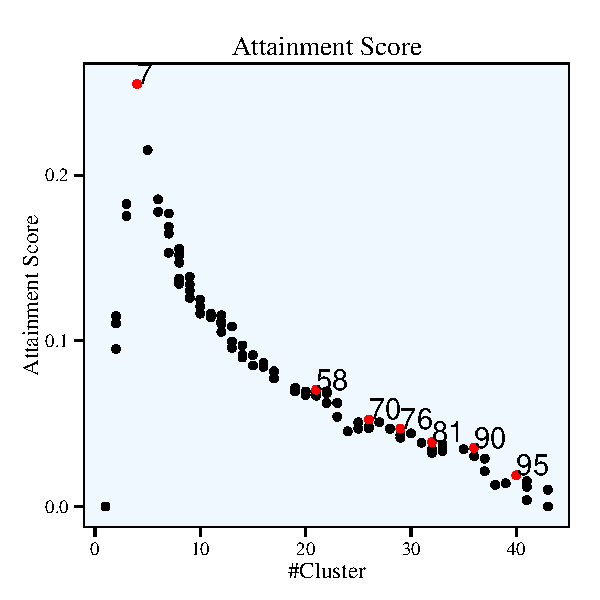
\includegraphics[width=\maxwidth]{figures/plots-attainment-1} 

}



\end{knitrout}
\caption{Attainment score with the global and local maxima}
\label{fig:attainment}
\end{center}
\end{figure}

\begin{figure}
\begin{center}
\begin{knitrout}
\definecolor{shadecolor}{rgb}{0.969, 0.969, 0.969}\color{fgcolor}

{\centering 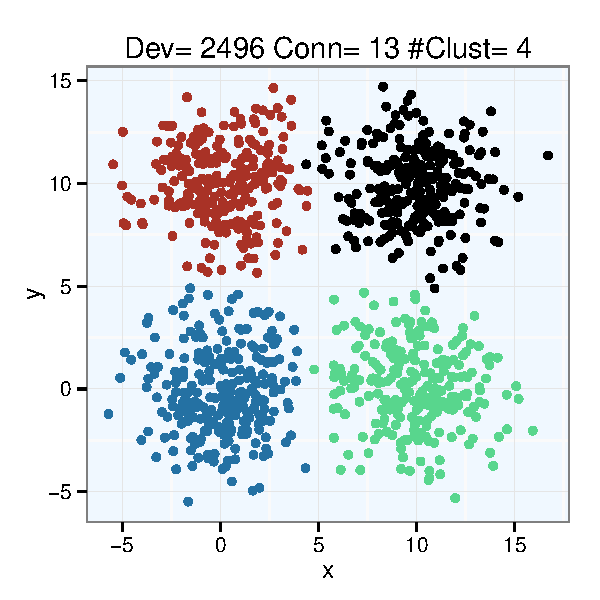
\includegraphics[width=\maxwidth]{figures/plots-clusterSolutions-1} 

}



\end{knitrout}
\caption{Visualization of the best solution for \textit{Square1} dataset}
\label{fig:best}
\end{center}
\end{figure}
has to be called. We can directly see the most promoising solutions visually indicated by their orange color with their corresponding solution index. If we now want to look at the best solution (see Figure \ref{fig:best}), we can simply plot solution number seven by calling:
\begin{knitrout}
\definecolor{shadecolor}{rgb}{0.969, 0.969, 0.969}\color{fgcolor}\begin{kframe}
\begin{alltt}
\hlkwd{printClusterSolution}\hlstd{(solution,}\hlnum{7}\hlstd{,square,}\hlnum{1}\hlstd{)}
\end{alltt}
\end{kframe}
\end{knitrout}



Now we can also run the same problem for a different algorithm like SMS-EMOA. Keep in mind that the parameters have to be adjusted accordingly. We again use the parameter setting of section 6:

\begin{knitrout}
\definecolor{shadecolor}{rgb}{0.969, 0.969, 0.969}\color{fgcolor}\begin{kframe}
\begin{alltt}
\hlstd{smsSolution} \hlkwb{=}  \hlkwd{mock}\hlstd{(}\hlkwc{data} \hlstd{= square,}\hlkwc{L} \hlstd{=} \hlnum{10}\hlstd{,}\hlkwc{crossRate} \hlstd{=} \hlnum{0.7}\hlstd{,}\hlkwc{nGrid} \hlstd{=} \hlnum{10}\hlstd{,}
                    \hlkwc{gens} \hlstd{=} \hlnum{10000}\hlstd{,}\hlkwc{method}\hlstd{=}\hlstr{"smsemoa"}\hlstd{,}\hlkwc{controlFronts} \hlstd{=} \hlnum{1}\hlstd{,}
                    \hlkwc{maxCluster}\hlstd{=}\hlnum{50}\hlstd{)}
\end{alltt}
\end{kframe}
\end{knitrout}



Now we have two solution objects. If we want to compare their pareto fronts (see Figure \ref{fig:multiple}) we can use another function within the MOCK package:
\begin{knitrout}
\definecolor{shadecolor}{rgb}{0.969, 0.969, 0.969}\color{fgcolor}\begin{kframe}
\begin{alltt}
\hlkwd{printMultipleParetoFronts}\hlstd{(}\hlkwd{list}\hlstd{(solution,smsSolution))}
\end{alltt}
\end{kframe}
\end{knitrout}


\begin{figure}
\begin{center}
\begin{knitrout}
\definecolor{shadecolor}{rgb}{0.969, 0.969, 0.969}\color{fgcolor}

{\centering 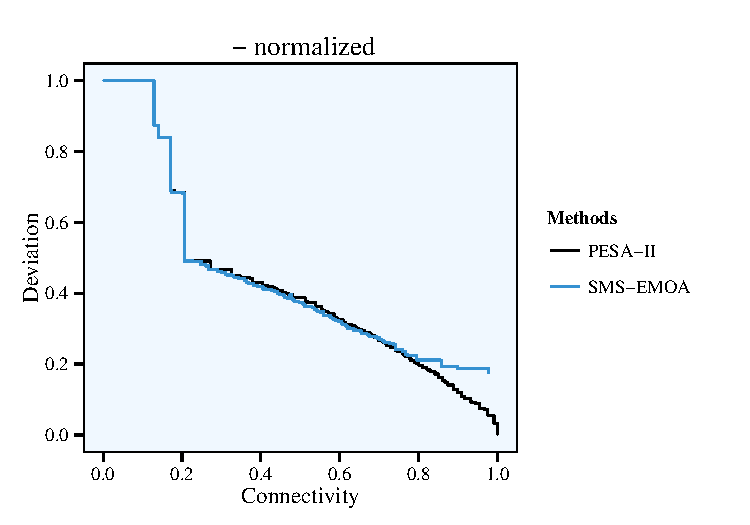
\includegraphics[width=\maxwidth]{figures/plots-printMultiple-1} 

}



\end{knitrout}
\caption{SMS-EMOA and PESA-II pareto fronts for the \textit{Square1} dataset}
\label{fig:multiple}
\end{center}
\end{figure}


\section{Outlook}
All in all the MOCK and PESA-II packages provide tools to analyze data structures efficiently. Next to PESA-II two additional EMOAs can be used for the clustering phase. Also it is possible to adapt other EMOAs by using the  recombination and mutation operators. A plethora of visualization methods allows the analyst to get a fast understanding of the underlying dara.

However in terms of the algorithm's runtime there is still space for improvements as it was already indicated within the implementation section. Although most of the crucial high volume functions were implemented in C++, especially the creation of many reference fronts is still pretty timeconsuming. Since the mock run on the clusterdata as well as the mock runs on the reference data are totally independend from each other, those runs can be parallelized. For upcoming versions of the package this feature is planned to be implemented with the highest priority. In regard to performance, no matter which EMOA is used for MOCK, the R implementation cannot compete with the speed of the original Mock tool. This is because the latter is implemented in C, a language much closer to machine language. After all the goal of the seminar was to provide an R implementation of MOCK, which currently does not exist, so that all the advantages could be gained. One of which is the integration of the package into R which allows easy pre- and post-processing and eliminates the effort to create an interface between the original Mock tool and other statistical computation tools.
\printbibliography
\end{document}
